\section{Prototype Constraints}
Before the prototype can be established, some considerations has to be made in respect to the time limitations and the main scope of this semester. The aim of the project is to create a functional proof of concept prototype of an automated lawn mower. The following section includes a brief description of the technology on which the prototype is constructed, along with argumentation for eliminated functionalities.

\subsection{Technology Base}
The technology which has been provided for the prototype is a tracked vehicle, seen on \figref{TrackedVehicle}. The vehicle comes with a brushed DC motor which provides power for rotation of the wheels, connected with the belts, and a servo motor which utilize breaks, connected to the wheels, to control the ratio of the differential steering. Furthermore the tracked vehicle includes two hall sensors, one by each belt, which keeps track of the speed, of the belts, by measuring pulses from magnets mounted on the front wheels. The testing will take place in Aalborg University Vicon Room, where the GoT system is installed and calibrated with the appurtenant transmitter, which is mounted on the tracked vehicle during test.

\begin{figure}[H]
	\centering
	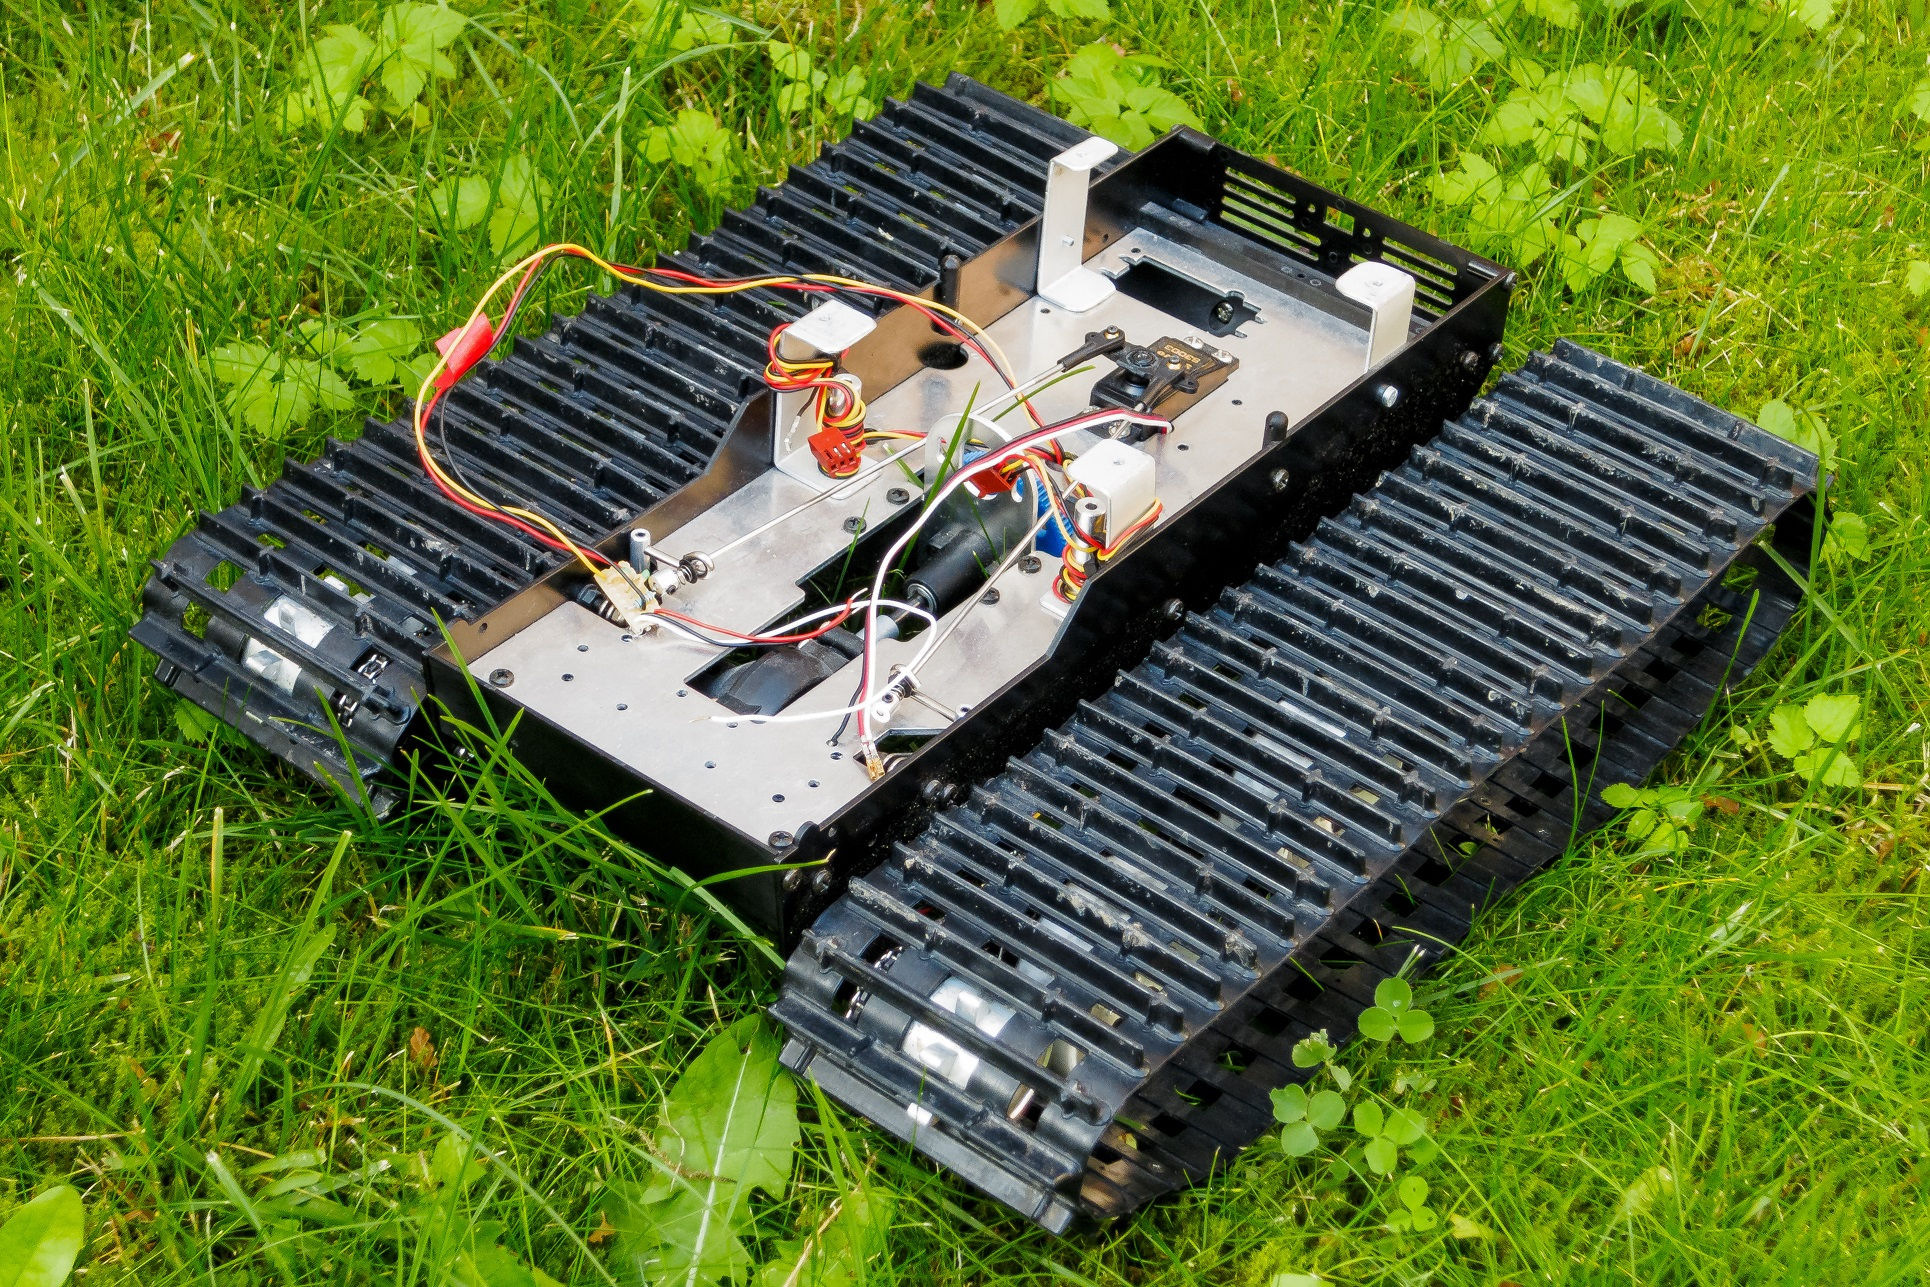
\includegraphics[scale=0.1]{figures/BeltVehicle.jpg}
	\flushleft
	\caption{The provided belt vehicle}
	\label{TrackedVehicle}
\end{figure}

\fxnote{datasheet of the vehicle}

\subsection{Grass Length Detection}
Detection of the grass length to control the speed of the lawn mower thus ensuring an evenly cut lawn, is a submodule which can be added at any time. Since it is not fatal for a working system and might even be unnecessary depending on time between each mowing of the lawn, it is decided to exclude this functionality from the initial design.

\subsection{Rain Sensor}
As the lawn mower is supposed to work outside, it is important to consider that it may be raining, and that an electronic device can be affected by those environmental issues. Even if the electrical part is waterproofed, there is a mechanical threat, a rain sensor could then warn the system to order the vehicle to get back in time.
It is possible to build the vehicle aware of those issues and add mechanical modules to secure it. However, the prototype will only be tested indoor, so this type of sensor will not be necessary in a prototype design.

\subsection{Obstacle Avoidance}
The lawn movers path might not always be clear, there could be some garden tools, tables or chairs, or people walking in it. The vehicle should be aware of what is in front of it at any time, to correct its path and get around the obstacle if necessary. To avoid this the sensor could be a pushing button to detect a solid strong object, or an ultrasound detector if the object is breakable.
As the aim of the project is to control the path of the vehicle by using angular positioning sensors, a proximity sensor will not be included. Static objects could be registered on the map to avoid these issues.\\\\
Furthermore the edge mapping functionality will not be included in the project which instead will focus on a quadratic map predefined in the test room.

\subsection{Power Monitoring}
Power monitoring could be implemented by measuring the voltage across the batteries, to ensure that the lawn mower is not running out of power, and to ensure the vehicles calculated route passes the charging station before the power runs too low.
This and the charging station will not be in the prototype, since it is beyond the scope of the project this semester and is not crucial for a working prototype.

\subsection{Prototype}
(to be continued)
%The overall functionalities for the project has been limited, due to time limitations and a desire to focus in the scope of the project. In this project a prototype will therefore be made to show the main functionalities necessary to make a automated vehicle.\\\\
%\noindent
%The final prototype is to contain a regulator which will make it possible to follow a path from A to B. It will be able to continue if the transmission is lost between the prototype and the GoT system for a while. Furthermore it should be able to store data points from the GoT system. (I think that it should be in more detail what the prototype should be able to do)

%%it used as an indoor prototype, and in worse case, the last position of the vehicle 
%%will be recorded. The user can then take it by hand and plug it into the charging
%%station.